\documentclass[12pt]{exam}
\newcommand{\hwnumber}{4}
\newcommand{\hwname}{Speller}
\newcommand{\duedate}{\formatdate{26}{09}{\YEAR} by \progDueTime} % day-month-year

\usepackage{../misc/latex/edition}  % Course semester
\usepackage{../misc/latex/c0}       % Listings style for c0
\usepackage{amsmath}
\usepackage{enumerate}
\usepackage[normalem]{ulem}
\usepackage{verbatim}
\usepackage[left=1in, right=1in, top=1in, bottom=1in]{geometry}
\usepackage{graphicx}
\usepackage{hyperref}
\usepackage{tikz}     \usetikzlibrary{shapes}
\usepackage{fancybox}
\usepackage[all]{xy}
\usepackage{wrapfig}
\usepackage{fancyvrb}
\usepackage{datetime}
\usepackage{etoolbox}
\usepackage{calc}
\usepackage[nomessages]{fp}
\usepackage{import}  % Like input and include, but respects subdirectories

\newcommand{\defaultQuestionLocation}{questions}
\newcommand{\inputQuestion}[2][\defaultQuestionLocation/]{%
  \subimport{#1}{#2}
}
% Subdirectories of \defaultQuestionLocation containing code and pictures
\newcommand{\code}{code}
\newcommand{\img}{img}


%%% ic: frontmatter macros
\newcommand{\specialInstructions}{}
\newcommand{\HWNUMBER}
{\ifdefempty{\hwnumber}{__}{%
  \ifnumless{\hwnumber}{10}{0\hwnumber}{\hwnumber}}}
\newcommand{\hwtype}{Written Homework}

%%% ic: 'exam' tweaks
\renewcommand{\half}{.5} % Half points

\newcommand{\Question}[2][]
 {\ifstrempty{#1}
    {\question{\bf #2}}
    {\question[#1]{\bf #2}}
  \immediate\write\rubricfile{}%
  \immediate\write\rubricfile{Question \thequestiontitle:}%
  \immediate\write\rubricfile{==========}
 }

%%% ic: Support for editable PDF
% counter name (some viewers misbehave if always the same)
\newcounter{editable}
\newcommand{\nextField}{\addtocounter{editable}{1}q\arabic{editable}}
\newcommand{\NextField}
 {\makebox[0pt][r]{\scalebox{0.1}{\color{White}\nextField}}}

% Color of edit area
\newcommand{\editAreaColor}{red}
% Single line answer:   \editableLine[extra parameters (optional)]{line width}
\newcommand{\editableLine}[2][]
{\textcolor{\editAreaColor}{%
 \underline{\hspace*{-0.25em}%
 \raisebox{-0.5ex}{%
 \TextField[width=#2, borderwidth=0, #1]{\NextField}}}}%
}
% Single line answer for code:  \editableLine[extra parameters (optional)]{line width}
\newcommand{\editableCodeLine}[2][]
{\textcolor{\editAreaColor}{%
 \underline{%
 \TextField[width=#2, height=1.5ex, borderwidth=0, #1]{\NextField}}}}
% Multiline answer:  \editableLine[extra parameters (optional)]{box height}
\newcommand{\editableBox}[2][]
{\leavevmode\hspace*{-0.1em}%
\TextField[height=#2, width=\linewidth,
           multiline=true, borderwidth=0.1, bordercolor=\editAreaColor,
           #1]{\NextField}}

%%%%% Same answer format as exams
\renewcommand{\rmdefault}{ppl}
\renewcommand{\sfdefault}{phv}
\newcommand{\answerColor}{Blue}

\ifprintanswers
\newcommand{\answer}[2]{\makebox[#1][c]{\color{\answerColor}#2}}
\else
\newcommand{\answer}[2]{\makebox[#1][c]{}\makebox[0pt]{\phantom{|}}}
\fi
\newcommand{\uanswer}[2]{\underline{\answer{#1}{#2}}}


%%% Write rubric snippet.  Usage:
% \RUBRIC
% any multi-line text (including \, #, %, whatever)
% ENDRUBRIC
%% (ENDRUBRIC should be on a line by itself)
\makeatletter
\def\RUBRIC
 {%
  \begingroup
  \let\do\@makeother\dospecials
  \endlinechar=`\^^J
  \@tofile%
 }
\def\ENDRUBRIC{ENDRUBRIC}
\def\@tofile#1^^J{%
  \def\@test{#1}%
  \ifx\@test\ENDRUBRIC
    \immediate\write\rubricfile{}  % End with an empty line
    \expandafter\@firstoftwo
  \else
    \expandafter\@secondoftwo
  \fi
  {\endgroup}%
  {\toks@{#1}%
   \begingroup\endlinechar=\m@ne
   \everyeof{\noexpand}%
   \xdef\@temp{\scantokens\expandafter{\the\toks@}}%
   \endgroup
   \immediate\write\rubricfile{\@temp}%
   \@tofile}%
}
\makeatother

%% Displays tags for an exercise in 'answer' mode
\newcommand{\TAGS}[1]
{\ifprintanswers%
  \rule{0em}{0ex}%
  \marginpar{\footnotesize%
    \fcolorbox{black}{Gray!25}{%
      \parbox[t]{2cm}{\raggedright\textbf{TAGS:}\\#1}}}%
  \ignorespaces%
 \fi}%


%% Page layout
\pagestyle{headandfoot}

\headrule
\header{\textbf{\courseNumber{} \hwtype{} \hwnumber}}
       {}
       {\textbf{Page \thepage\ of \numpages}}
\footrule
\footer{}{}{\COPYRIGHT}

\renewcommand{\partlabel}{\textbf{\thequestion.\thepartno}}
%\renewcommand{\partlabel}{\textbf{Task \thepartno}}
\renewcommand{\subpartlabel}{\textbf{\thesubpart.}}
\renewcommand{\thepartno}{\arabic{partno}}
\renewcommand{\thesubpart}{\alph{subpart}}
\pointpoints{pt}{pts}
\pointformat{\raisebox{0ex}[\height][0pt]{\fcolorbox{black}{yellow}{\themarginpoints}}}
\bonuspointformat{\raisebox{0ex}[\height][0pt]{\fcolorbox{black}{red}{\themarginpoints}}}
\marginpointname{\points}
\pointsinmargin
%\boxedpoints

\setlength\answerlinelength{2in}
\setlength\answerskip{0.3in}

\newcommand{\mkWrittenTitle}[1]{#1}
\newcommand{\mkDueDate}[1]{#1}
\newcommand{\mkEvalSummary}[1]{#1}
\newcommand{\mkGradetable}[1]{#1}



% This fixes an issue with the exam package version 2.6 and after,
% where 'framed' has been renamed to 'examframed' to avoid a conflict.
\ifcsmacro{examframed}{%
\newenvironment{framed}
{\begin{examframed}}
{\end{examframed}}
}{}

\begin{document}
\hwTitle

\noindent
This week we will do some relatively small exercises centered around
searching and sorting arrays of integers and strings. We compared
characters and strings for equality during the puzzle hunt portion of
our first programming assignment; Appendix~\ref{sec:strings} of this
writeup talks a little big more about string comparison, which is
necessary when we think about sorted arrays of strings.

\bigskip
\noindent
The code handout for this assignment is on \autolab{} and at
\begin{center}
\whereisthetgz{speller-handout.tgz}
\end{center}
The file \lstinline'README.txt' in the code handout goes over the contents
of the handout and explains how to hand the assignment in.

\bigskip
\noindent
There is a FIVE (5) PENALTY-FREE HANDIN LIMIT.  Every additional
handin will incur a small (5\%) penalty (even if using a late day).
{\bf Be aware that only Task~7 will be graded by Autolab when you hand
  in your work. You should examine Autolab's output to make sure the
  other tasks compile. \emph{If you don't check Autolab's outputs and
    there are compilation errors, you may end up receiving no credit
    for the assignment.}}

The other tasks will be autograded or graded by hand after the
assignment deadline. You will need to use the test cases you write for
task 7, contracts, and deliberate programming to ensure correctness of
the other tasks.

\newpage
\section{Introduction}
\label{sect:common}

\paragraph{The story:} %
The Hackers from the Lost Web, a cyber-criminal organization that
specializes in ransomware, has disabled all spellchecking software on
campus.
% A horrible calamity has befallen CMU's campus and every single
% instance of spellchecking software on campus has disappeared.
You have a term paper due and you are worried your professor will
lower your grade if there are spelling mistakes in your paper. Being a
15-122 student, you decide to write your own spellchecker with the
help of the friendly 15-122 staff.

\paragraph{Your tools:} %
Your diligent 15-122 TA's have given you a C0 library for reading text
files, converting all letters to lowercase, and separating out
words. It is provided to you as \lstinline'lib/readfile.c0', which
defines a type \lstinline'bundle_t' and implements the following
functions:

\begin{quote}
\begin{lstlisting}[basicstyle=\smallbasicstyle]
// First call read_words to read in the content of the file
bundle_t read_words(string filename)
\end{lstlisting}
\end{quote}
You don't need to understand anything about the type
\lstinline'bundle_t' other than that you can extract its underlying
\lstinline'string' array and the length of that array:
\begin{quote}
\begin{lstlisting}[basicstyle=\smallbasicstyle]
// To determine the length of the array in the string_bundle, use:
int string_bundle_length(bundle_t sb)

// Access the array inside of the string_bundle using:
string[] string_bundle_array(bundle_t sb)
//@ensures \length(\result) == string_bundle_length(sb);
\end{lstlisting}
\end{quote}

\noindent
Here's an example of these functions being used on a tweet by local
weatherman Scott Harbaugh:

\begin{center}
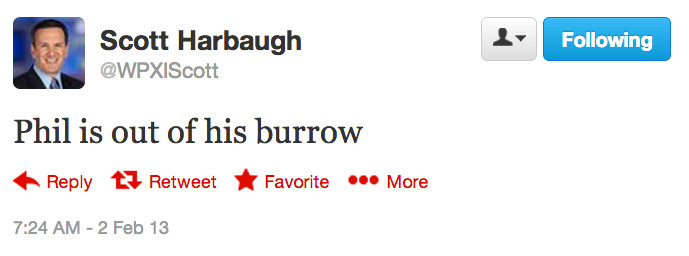
\includegraphics[width=0.7\textwidth]{img/wpxiscott.png}
\end{center}


\begin{quote}
\begin{lstlisting}[language={[coin]C}, basicstyle=\smallbasicstyle]
% coin -d lib/readfile.c0
--> bundle_t B = read_words("texts/scott-tweet.txt");
B is 0x7047F0 (struct string_bundle_header*)
--> string_bundle_length(B);
6 (int)
--> string[] tweet = string_bundle_array(B);
tweet is 0x704B60 (string[] with 6 elements)
--> tweet[0];
"phil" (string)
--> tweet[5];
"burrow" (string)
\end{lstlisting}
\end{quote}

\paragraph{Your data:} You are given you 2 dictionaries and 3 text
files for your project in the \lstinline'texts/' directory:
\begin{itemize}
\itemsep=0pt
\item \lstinline'dict.txt' --- %
  A standard dictionary you will be using.
\item \lstinline'small-dict.txt' --- %
  A minuscule dictionary.
\item \lstinline'scott-tweet.txt' --- %
  A tiny text file: Scott Harbaugh's tweet.
\item \lstinline'sloth.txt' --- %
  Another small text file: the sloth example below.
% \item \lstinline'sonnets.txt' --- %
%   A medium text file: 122 of Shakespeare's sonnets.
\item \lstinline'shakespeare.txt' --- %
  A larger text file: the complete works of Shakespeare.
\end{itemize}
You can write more data files of your own!


\section{Spellchecking a Word}

In this exercise, you will write a binary search function for
spellchecking a word against a dictionary.  The dictionary is
represented as a sorted array \lstinline'dict' of strings and has
length \lstinline'd', while the word is represented as a string
\lstinline'w'.  The function \lstinline'check_word' that you will
write returns a boolean value indicating whether \lstinline'w' is in
the dictionary.

For example, we expect that \lstinline'check_word(dict, d, "sloth")'
returns \lstinline'true' while %
\lstinline'check_word(dict, d, "sloathe")' %
returns \lstinline'false' with respect to the standard dictionary
(file \lstinline'dict.txt').

The code for this exercise should be put in a file
\lstinline'speller.c0'. You must include annotations for the
precondition(s), postcondition(s) and loop invariant(s) for each
function.  Include additional annotations for assertions as necessary.
You may put any auxiliary functions you need in the same file, but you
should \emph{not} include a \lstinline'main()' function.  You can use
functions from the \lstinline'lib/readfile.c0' file in your code.

\begin{task}[2]
\TAGS{array, complexity, divide-and-conquer, safety, search, sorting}
Implement the function \lstinline'check_word' in file
\lstinline'speller.c0':
%\begin{quote}
\begin{lstlisting}[basicstyle=\smallbasicstyle]
bool check_word(string[] dict, int d, string w)
//@requires \length(dict) == d;
//@requires is_sorted(dict, 0, d) && no_dupes(dict, 0, d);
\end{lstlisting}
%//@ensures \result == true ? is_in(w,dict,0,d) : !is_in(s,dict,0,d);
%\end{quote}
This function should return whether the word \lstinline'w' is in the
dictionary \lstinline'dict'. The preconditions let you assume that the
dictionary \lstinline'dict' is sorted and has no duplicates, a fact
you should exploit for your code to run in time $O(\log d)$ --- and
implementation based on linear search is likely to fail subsequent
tasks.
\end{task}


\section{Spellchecking a Text}

Now that we are able to spellcheck a word, let's spellcheck a whole
text.  Consider this text:

\begin{quote}\sloppypar\tt\small
  Sloths are named after the capital sin of sloth; however, their
  usual idlleness is due to metabolic adaptations for conserving
  energie. Aside from their surprising speed during emergency flights
  from predators, other notable traits of sloths include their strong
  body and their ability to host symbiotic algee on their furs.
\end{quote}

\subsection{Word by Word}

An obvious way to spellcheck this text is to first call
\lstinline'check_word(dict, d, "sloths")' and then call
\lstinline'check_word(dict, d, "are")' and so on.  Let's automate this
idea by storing the text in an array of strings, one word in each
location, and calling \lstinline'check_word' inside a loop that
iterates over each word.  Rather than just returning whether the whole
text was or wasn't correctly spelled, our spelling functions will
return an array containing all the misspelled words in the text.

\begin{task}[2]
\TAGS{array, correctness, loop-invariant, safety, search}
In \lstinline'speller.c0', complete the definition of the function
\begin{lstlisting}[basicstyle=\smallbasicstyle]
int check_text_naive(string[] dict, int d, string[] text, int t, string[] miss)
//@requires \length(dict) == d;
//@requires \length(text) == t;
//@requires \length(miss) >= t;
//@requires is_sorted(dict, 0, d) && no_dupes(dict, 0, d);
//@ensures 0 <= \result && \result <= t;
//@ensures no_dupes(miss, 0, \result);
\end{lstlisting}
The function takes in five arguments. The first two are the dictionary
(which is sorted and has no duplicates) and its length. The next two
are the text you are spellchecking and its length. The final argument,
\lstinline'miss', is the array that you will use to return the
misspelled words you find. This array needs to be at least as big as
the text array because every word might be misspelled.  As you find
misspelled words, you will write each of them in order into the array
\lstinline'miss', starting at index 0, without repetitions.  The
function returns the number of words you wrote into \lstinline'miss',
i.e., the number of unique misspelled words in the text.  Later on in
this course, we will learn more elegant ways of returning two pieces
of data from a function.  For example, for the text given earlier, the
\lstinline'miss' array should contain the strings \lstinline'idlleness',
\lstinline'energie' and \lstinline'algee' (in that order in the
first three slots) and \lstinline'\result' should be equal to 3.
\end{task}


\subsection{Spellchecking Sorted Texts without Duplicates}

The complexity of \lstinline'check_text_naive' is at least $O(t \log
d)$ because it calls \lstinline'check_word' (which has cost $O(\log
d)$) on each of the $t$ words in the text.\footnote{It's actually even
  worse given that the \lstinline[basicstyle=\smallerbasicstyle]'miss' array shall not contain
  duplicates.}  You can easily see from our example that we will end
up spellchecking common words like \lstinline'sloths', \lstinline'are'
and \lstinline'their' multiple times.  A text without duplicates is
clearly immune from this problem.  The cost is still $O(t \log d)$
however.  \emph{Can we do better?}

The 15-122 TAs unanimously claim \textbf{\em we can} if the text is
\emph{sorted}!  They give you the challenge to implement a
spellchecker for sorted texts without duplicates that runs in time
$O(\max(d,t))$ --- and doesn't use \lstinline'check_word'.

\newpage
\begin{task}[4]
\TAGS{array, correctness, loop-invariant, safety, search, sorting}
In \lstinline'speller.c0', complete the definition of the function
\begin{lstlisting}[basicstyle=\smallbasicstyle]
int check_sorted_text(string[] dict, int d, string[] text, int t, string[] miss)
//@requires \length(dict) == d;
//@requires \length(text) >= t;
//@requires \length(miss) >= t;
//@requires is_sorted(dict, 0, d) && no_dupes(dict, 0, d);
//@requires is_sorted(text, 0, t) && no_dupes(text, 0, t);
//@ensures 0 <= \result && \result <= t;
//@ensures is_sorted(miss, 0, \result) && no_dupes(miss, 0, \result);
\end{lstlisting}
You should spellcheck only the first \lstinline't' words of
\lstinline'text' (why will become clear later).  As before, the
function should return the number of misspelled words, and you should
populate the array \lstinline'miss' with those words.  Since the text
is sorted, so will the computed misspelled words.  Make sure that the
running time of this function is indeed $O(\max(d,t))$ as it may time
out on Autolab otherwise.
\end{task}


\subsection{Sorting a Text and Removing Duplicates}

But everyday texts like essays and email are not sorted and they do
contain duplicates.  Our next task will be to take such a text and
generate another text that is sorted and contains the same words, only
once.

One convenient way to remove duplicates is while sorting the text
array.  For example:
\begin{center}
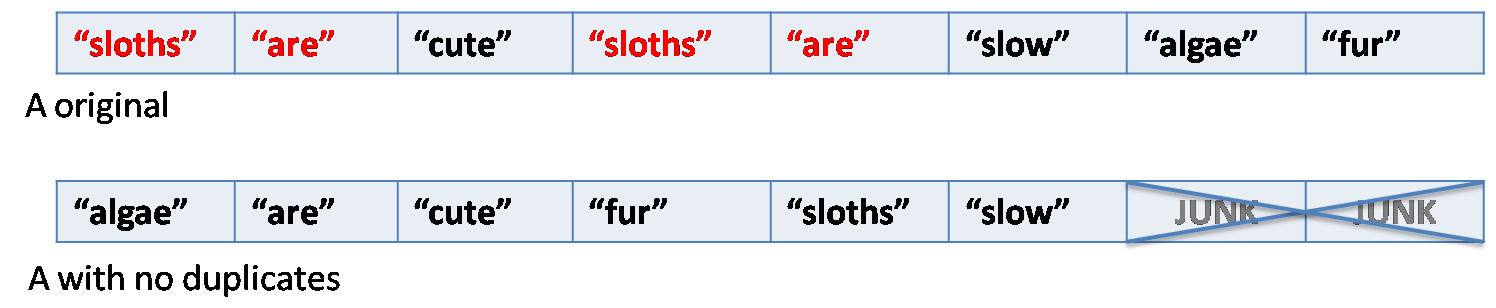
\includegraphics[width=0.7\textwidth]{img/dupes.png}
\end{center}
As you can see, the array \lstinline'A' has length 8, but there are
two duplicates in the array (highlighted in red).  If we sort and
remove the duplicates, we get an array that is still of size 8, but
only the first 6 slots have values we actually care about.

For full credit on the next two tasks, you will need to write a
sorting algorithm that is \textbf{fast} and \textbf{removes
  duplicates}.  By fast, we mean that it will be $O(t \log t)$ on a
$t$-word input text.  The easiest way to make a fast,
duplicate-removing sort is to modify mergesort, which we talked about
in class; code for mergesort is published alongside the lecture notes
on divide-and-conquer sorting.  We advise you to look into this code
and to work out some examples before you move on to modifying
mergesort.

In order to cleanly remove duplicates and keep track of the number of
unique elements in the array, we have rewritten the prototypes of
mergesort as follows:

\begin{lstlisting}[basicstyle=\smallbasicstyle]
int merge(string[] A, int lo1, int hi1, int lo2, int hi2)
//@requires 0 <= lo1 && lo1 < hi1 && hi1 <= lo2 && lo2 < hi2 && hi2 <= \length(A);
//@requires is_sorted(A, lo1, hi1) && no_dupes(A, lo1, hi1);
//@requires is_sorted(A, lo2, hi2) && no_dupes(A, lo2, hi2);
//@ensures 0 <= \result && \result <= hi2 - lo1;
//@ensures is_sorted(A, lo1, lo1 + \result) && no_dupes(A, lo1, lo1 + \result);
\end{lstlisting}

\begin{lstlisting}[basicstyle=\smallbasicstyle]
int mergesort(string[] A, int lo, int hi)
//@requires 0 <= lo && lo <= hi && hi <= \length(A);
//@ensures 0 <= \result && \result <= hi - lo;
//@ensures is_sorted(A, lo, lo + \result) && no_dupes(A, lo, lo + \result);
\end{lstlisting}


These functions now return an \lstinline'int' instead of
\lstinline'void' because we will use this value to keep track of the
number of unique elements in the resulting array.  The arguments to
\lstinline'mergesort' are the same as those in the standard mergesort
implementation. However, you will notice that our \lstinline'merge'
function takes four array indices as arguments instead of
three.  Instead of passing it \lstinline'lo', \lstinline'mid' and
\lstinline'hi', we pass it two sorted intervals \lstinline'[lo1, hi1)'
and \lstinline'[lo2, hi2)' that contain no duplicates that we need to
merge together. We can't use a standard \lstinline'merge' because
it would merge the junk at the end of each segment into the output
array.

For example, after we call \lstinline'merge(B, 0, 3, 4, 8)' on the
array \lstinline'B' pictured below, the array \lstinline'B' will
contain the merged and sorted intervals, and return 6.

\begin{center}
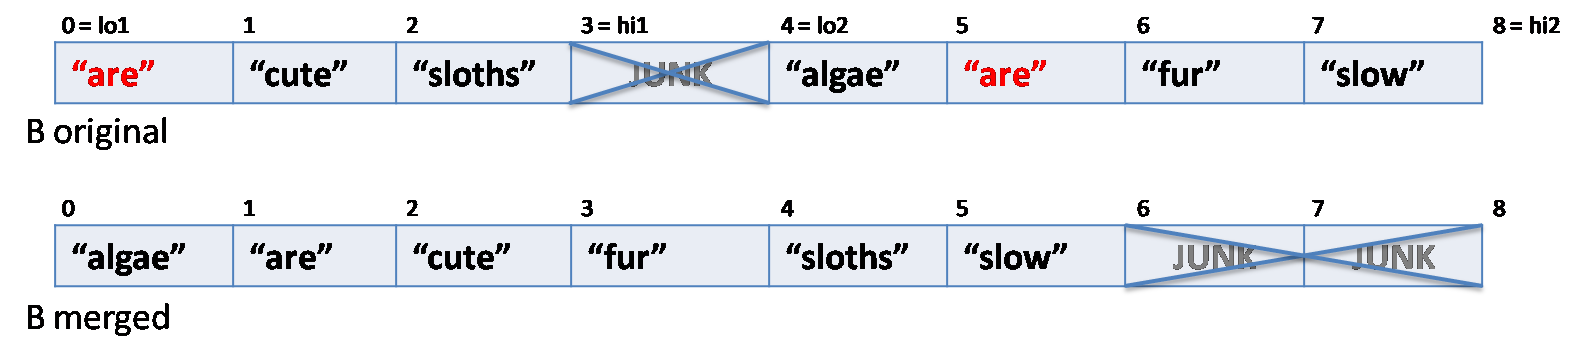
\includegraphics[width=0.7\textwidth]{img/merge.png}
\end{center}

Your next job is to first implement \lstinline'merge' and then
\lstinline'mergesort'. Make sure you test your mergesort
implementation to ensure it is removing duplicates.

\begin{task}[5]
\TAGS{array, correctness, loop-invariant, safety, sorting}
Add to \lstinline'speller.c0' a definition of the function
\lstinline'merge' as defined above.
\end{task}

\begin{task}[3]
\TAGS{array, correctness, loop-invariant, safety, sorting}
Add to \lstinline'speller.c0' a definition of the function
\lstinline'mergesort' as defined above.
\end{task}


\subsection{Better Spellchecking}

With a way to sort and remove duplicates from a text and a way to
quickly spellcheck a text with these characteristics, we can write a
spellchecker for a generic text that, in many cases, runs faster than
\lstinline'check_text_naive'.

\begin{task}[2]
\TAGS{array, correctness, loop-invariant, safety, search, sorting}
Add to \lstinline'speller.c0' a definition of the function
\lstinline'check_text_better' that first sorts a text and then
spellchecks it.
\begin{lstlisting}[basicstyle=\smallbasicstyle]
int check_text_better(string[] dict, int d, string[] text, int t, string[] miss)
//@requires \length(dict) == d;
//@requires \length(text) == t;
//@requires \length(miss) >= t;
//@requires is_sorted(dict, 0, d) && no_dupes(dict, 0, d);
//@ensures 0 <= \result && \result <= t;
//@ensures  is_sorted(miss, 0, \result) && no_dupes(miss, 0, \result);
\end{lstlisting}
As always, the function should return the number of misspelled words,
and you should populate the array \lstinline'miss' with those words,
in alphabetical order.
\end{task}


\newpage
\section{Unit Testing}
\label{ref:unit-test}

The functions you wrote in the earlier tasks could fail in many
ways. On certain inputs, they might fail internal assertions or
postconditions (\emph{contract failures}), and on other inputs they
might happily return invalid results (\emph{contract exploits}).

\begin{task}[4]
\TAGS{testing}
\label{task:unit-test}
Write a file, \lstinline'speller-test.c0', that tests your
implementation of your \lstinline'check_word' and
\lstinline'check_text_better'.  Your \lstinline'speller-test.c0'
should test \textbf{only} these two functions.  Do not assume the
existence of \lstinline'merge', \lstinline'mergesort',
\lstinline'check_text_naive', or \lstinline'check_sorted_text'.  The
autograder will assign you a grade based on the ability of your unit
tests to pass when given a correct implementation and fail when given
various buggy implementations.  Your tests must still be safe: it
should not be possible for your code to make an array access
out-of-bounds when \lstinline'-d' is turned on.

  You do not need to catch all our bugs to get full points, but
  catching additional tests will be reflected on the scoreboard.
\end{task}

Because you cannot access all of our buggy implementations except via
the autograder, your grade on this task \emph{will} be given as soon
as you hand in your work.
We'll run tests with contracts (\lstinline'-d') enabled, so the largest
text files should not be used in your unit tests.

You may find it useful to use the functions provided in C0's
\lstinline'parse' library. These functions provide a convenient way
of creating arrays with specific contents.  It's not necessary to use
this library to test your code, but you may find that writing
\begin{quote}
\begin{lstlisting}[belowskip=0pt, basicstyle=\smallbasicstyle]
string[] A = parse_tokens("I love 15-122");
\end{lstlisting}
\end{quote}
is more convenient than writing
\begin{quote}
\begin{lstlisting}[belowskip=0pt, basicstyle=\smallbasicstyle]
string[] A = alloc_array(string, 3);
A[0] = "I";
A[1] = "love";
A[2] = "15-122";
\end{lstlisting}
\end{quote}


\subsubsection*{Testing your tests}
You can test your functions with your own implementation, and with an
awful and badly broken implementation, by running the following
commands:

\begin{quote}
\begin{lstlisting}[language={[coin]C}, aboveskip=1pt, belowskip=0pt, basicstyle=\smallbasicstyle]
% cc0 -d -w lib/*.c0 speller.c0 speller-test.c0
% ./a.out
% cc0 -d -w lib/*.c0 speller-awful.c0 speller-test.c0
% ./a.out
\end{lstlisting}
\end{quote}
Both tests should compile and run, but the last invocation of
\lstinline'./a.out' should trigger a assertion to fail if your tests are
more than minimal. \emph{Even if your test cases fail on the
  awful implementation, they still might not be particularly useful
  test cases.}



\newpage
\section{Analyzing the Results}
\newcommand{\redacted}
 {\underline{\hspace{1.5em}}\mathtt{REDACTED}\underline{\hspace{1.5em}}}

Once you've carefully tested your \lstinline'speller.c0' implementations,
you have a powerful set of tools for analyzing your input text. For
the last part of this assignment, you'll run such an analysis.
\emph{It is a violation of the academic integrity policy of this
  course to compare the answers in this section with other students.}

\begin{task}[3]
\TAGS{application, testing}
Create a file \lstinline'analysis.c0' containing a
\lstinline'main()' function.  Here's how to compile and an example
of how to run this file:
\begin{quote}
\begin{lstlisting}[language={[coin]C}, basicstyle=\smallbasicstyle]
% cc0 -w -o analysis lib/*.c0 speller.c0 analysis.c0
% ./analysis texts/dict.txt texts/shakespeare.txt
\end{lstlisting}
\end{quote}
The first argument to the function is the filename for the (sorted)
dictionary and the second argument is the text.  See
\lstinline'echo.c0' for an example of how to handle command-line
arguments in C0.  Note that, to receive credit, your implementation
shall work for an arbitrary dictionary and an arbitrary text ---
possibly much larger than the above example --- passed as parameters
as above.

Your analysis should compute and print out human-readable answers to
the following questions:

\begin{itemize}
\itemsep=0pt
\item%
  How many unique misspelled words are there in the text (relative to the
  dictionary)?
\item%
  How many unique misspelled words of length exactly 8 are there in the text
  relative to the dictionary?
\item%
  List alphabetically the first 4 misspelled words of length 15 in the
  text relative to the dictionary.
\item%
  How many times does the alphabetically-last misspelled word (this
  would be ``idlleness'' in the sloth example) appear
  in the text?  If the text does not contain misspelled words, point
  this out.
\end{itemize}
Your code only needs to work on reasonable inputs. Specifically, don't
worry about checking that the first argument is a file of words that
are actually sorted. If you use the tools you developed in this
assignment correctly, you should be able to compute the answers from
scratch in a couple of seconds.
\end{task}
\enlargethispage{5ex}
We don't need the output of your analysis to obey a strict format, but
here's the rough format you should follow:
\begin{quote}
\begin{lstlisting}[language={[coin]C}, mathescape, aboveskip=0pt, basicstyle=\smallbasicstyle]

There are $\redacted$ misspelled words in the text.

There are $\redacted$ misspelled words of length 8 in the text.

Here are the first 4 misspelled words of length 15 in the text:
 1. $\redacted$
 2. $\redacted$
 3. $\redacted$
 4. $\redacted$

The alphabetically-last misspelled word in the text is $\redacted$ and
appears $\redacted$ times.
\end{lstlisting}
\end{quote}

\newpage
\appendix
\section{String Processing Overview}
\label{sec:strings}

In the C0 language, a \lstinline'string' is a sequence of
characters. Unlike languages like C, a string is not the same as an
array of characters. One of the functions in the string library
(which you include in your code by \lstinline+#use <string>+) is
\lstinline'string_compare':
\begin{quote}
\begin{lstlisting}[basicstyle=\smallbasicstyle]
int string_compare(string a, string b)
//@ensures -1 <= \result && \result <= 1;
\end{lstlisting}
\end{quote}
The \lstinline'string_compare' function performs a
\emph{lexicographic} comparison of two strings, which is essentially
the ordering used in a dictionary, but with character comparisons
being based on the characters' ASCII codes, not just alphabetical. We
can convert back and forth between the \lstinline'char' type and the
integer ASCII codes with the \lstinline'char_ord(c)' and
\lstinline'char_chr(i)' functions, also available in the string
library.  For this reason, the ordering used here is sometimes
whimsically referred to as ``ASCIIbetical'' order.  A table of all the
ASCII codes is shown in Figure~\ref{fig:asciitable}.  The ASCII value
for \texttt{'0'} is \lstinline'0x30' (48 in decimal), the ASCII code
for \texttt{'A'} is \lstinline'0x41' (65 in decimal) and the ASCII
code for \texttt{'a'} is \lstinline'0x61' (97 in decimal). Note that
ASCII codes are set up so the character \texttt{'A'} is ``less than''
the character \texttt{'B'} which is less than the character
\texttt{'C'} and so on, so the ``ASCIIbetical'' order coincides
roughly with ordinary alphabetical order.

\bigskip
\bigskip

\begin{figure}[hb]
\centering
    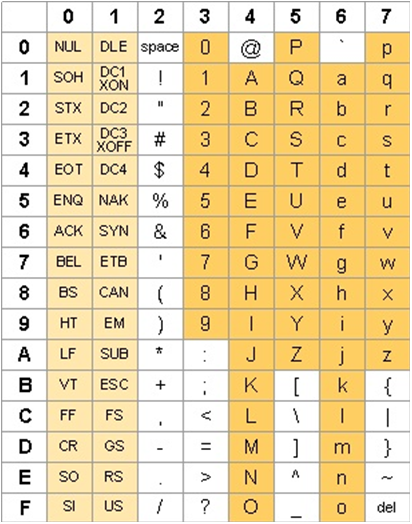
\includegraphics[width=80mm]{img/asciitable.png}
\caption{The ASCII table}
\label{fig:asciitable}
\end{figure}


\end{document}
